% !TeX spellcheck = da_DK
\subsection{Accelerometer}\label{Acc_afsnit}
\subsubsection{Teori og design}
Teorien og specifikationer vedrørende accelerometret ADXL$335$ er i afsnit \ref{Subsec:AccTeori} på side \pageref{Subsec:AccTeori}. Designet af opsætningen kan ses i bilag \ref{Bilag:Pilotforsoeg}, side \pageref{Bilag:Pilotforsoeg} med en ændring af den ene kondensator. I pilotforsøget blev det påvist, at signalet ligger mellem $0-25$Hz, og derfor benyttes en kondensator med en anden kapacitans fremfor den kondensator, der blev brugt i pilotforsøget \cite{Devices2009}:
\begin{equation}
\text{Båndbredde} = \dfrac{5\mu F}{C} \Rightarrow  C = \dfrac{5\mu F}{\text{25 Hz}} = 0.2\mu F
\end{equation}
For at undgå loading fra andre blokke i systemet benyttes en buffer, jævnfør bilag \ref{Bilag:Pilotforsoeg}, side \pageref{Bilag:Pilotforsoeg}. Til bufferkonfigurationen bruges en operationsforstærker af typen TL$081$, hvis pinkonfiguraion kan ses på \figref{fig:TL081}. 

\begin{figure}[H]
	\centering
	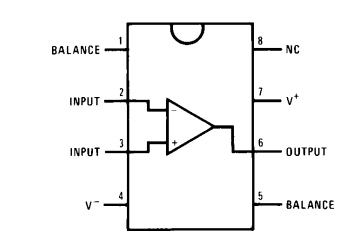
\includegraphics[scale=.8]{figures/cProblemloesning/TL081.PNG}
	\caption{På figuren ses pinkonfigurationen for operationsforstærkeren TL$081$.\cite{Corporation1995}}
	\label{fig:TL081}
\end{figure}

\subsubsection{Simulering}
Jævnfør tolerancekravene for accelerometret beskrevet i afsnit \ref{OpsamlingsAfs} på side \pageref{OpsamlingsAfs} skal der testes for, hvorledes accelerometret overholder kravet om, at der maksimum må være en $5\%$ afvigelse i detektionen af hældningsgrad. \\
Der findes ikke et accelerometer i LTspice, hvorfor accelerometeret er symboliseret med en sinuskurve. Dets DC svarer til spændingsforsyning $5.5$V fratrukket offsettet for accelerometeret ved $0$g påvirkning, som er $1.6325$V. Derudover angives en amplitude svarende til den maksimale sensitivitet på $0.3313$V. Simuleringen ses på \figref{fig:acc_simulering} og resultatet ses på \figref{fig:acc_simulering_resultat}.
\begin{figure}[H]
	\centering
	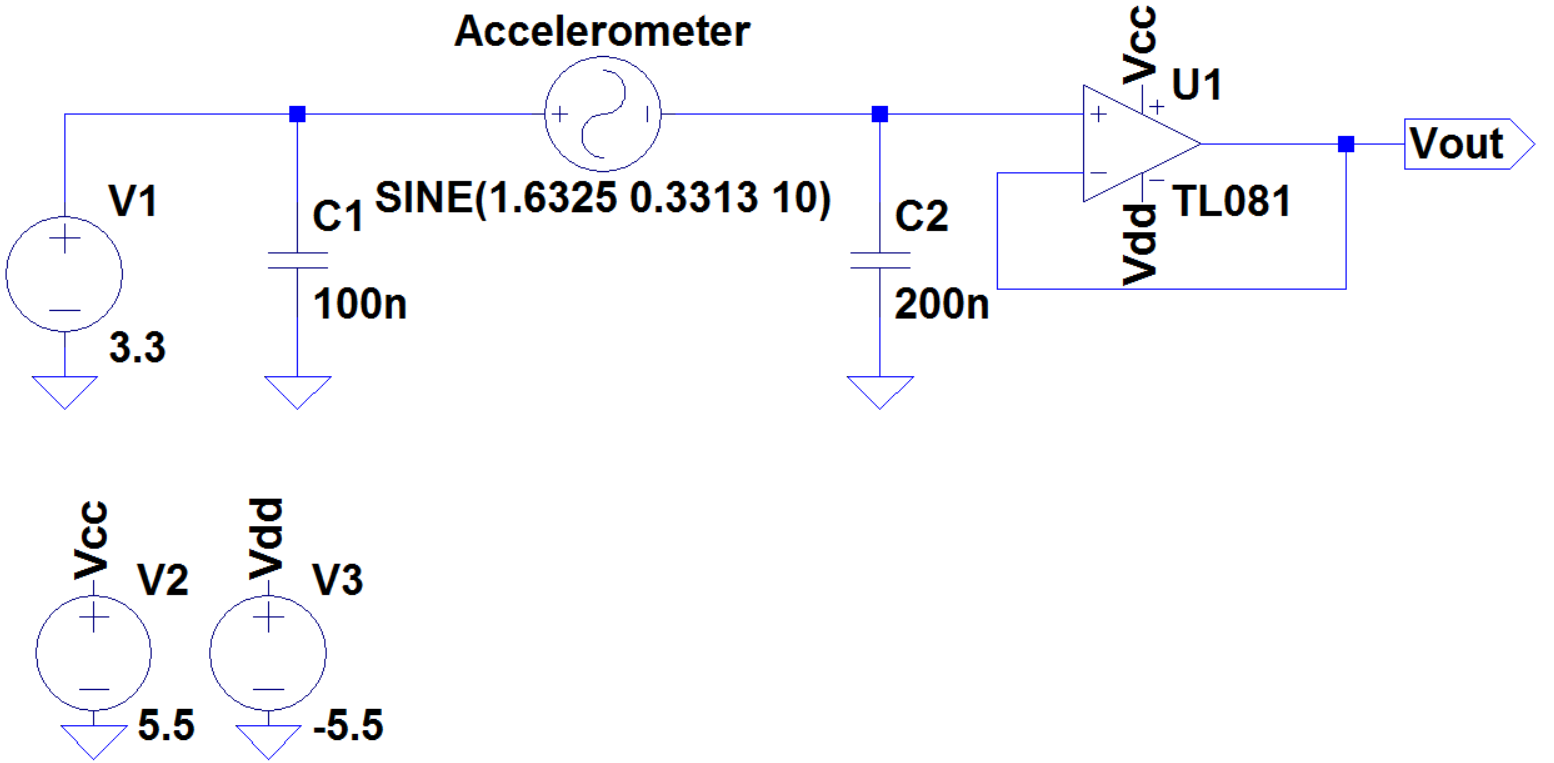
\includegraphics[scale=.4]{figures/cProblemloesning/Acc_Simulering1.PNG}
	\caption{På figuren ses designet af accelerometret i opsamlingsblokken i LTspice. Accerometeret er erstattet med en sinuskurve med et offset på $1.6325$V ($3.3$V-$1.6325$V=$1.6675$). Derudover indstilles amplituden til accelerometerets sensitivitet $0.3313$V og frekvensen til $10$Hz. På figures ses en buffer implementeret til outputtet for at forhindre loading, som er beskrevet og forklaret i bilag \ref{Bilag:Pilotforsoeg}, side \pageref{Bilag:Pilotforsoeg}.}
	\label{fig:acc_simulering}
\end{figure}
\begin{figure}[H]
	\centering
	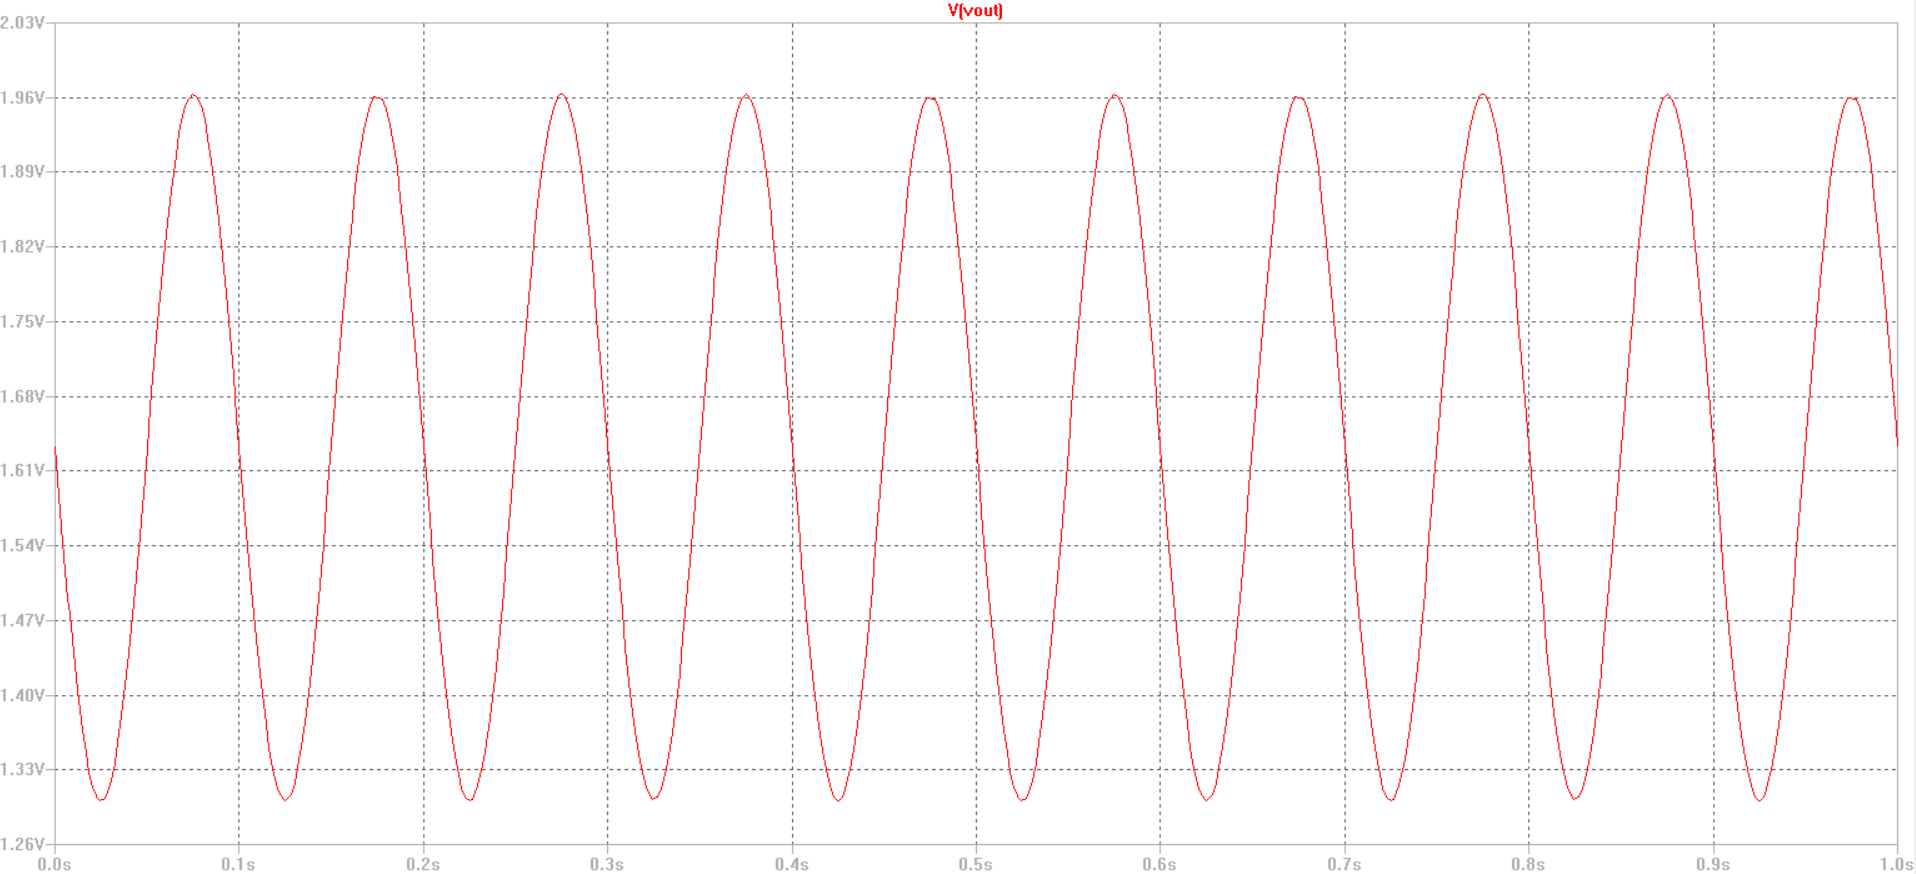
\includegraphics[scale=.38]{figures/cProblemloesning/Acc_Simulering2.PNG}
	\caption{På figuren ses simuleringen af accelerometret som en sinus med et offset på $1.6325$V, amplitude på $0.3313$V og frekvensen er $10$Hz. Der ses, at $V_{out}$ maksimalt er ca. $1.96$V og minimalt ca. $1.30$V.}
	\label{fig:acc_simulering_resultat}
\end{figure}

\subsubsection{Implementering og test}
%I pilotforsøget bliver der arbejdet med reelle komponenter, hvilket også bliver benyttet til implementeringen. Derfor antages det, at der vil være en mindre afvigelse imellem resultaterne fra testen og pilotforsøget end imellem resultaterne fra testen og en eventuel simulering, da der i simuleringer arbejdes med ideelle komponenter.
Accelerometerets båndbredde bestemmes af to $0.1\mu$F kondensatorer i parallelforbindelse, som derved vil give en samlet kapacitans på  $0.2\mu$F. De tre kondensatorer samt den samlede kapacitans måles inden implementering. Resultaterne fremgår i  \tableref{Tab:Acc_kondensator}:
\begin{table}[H]
	\centering
	\begin{tabular}{|l|l|l|l|} \cline{2-4} \multicolumn{1}{l|}{} & \textit{Teoretisk} & \textit{Målt} & \textit{\% afvigelse} \\ \hline
		\textit{C1}       & \textit{$0.1\mu$F} & $0.1004\mu$F  & $0.4\%$               \\ \hline		
		\textit{C2}       & \textit{$0.1\mu$F} & $0.1009\mu$F  & $0.9\%$               \\ \hline
		\textit{C3}       & \textit{$0.1\mu$F} & $0.0989\mu$F  & $1.1\%$               \\ \hline
		\textit{$C_{eq}$ af C2 || C3} & \textit{$0.2\mu$F} & $0.2002\mu$F  & $1\%$                \\ \hline
	\end{tabular}
	\caption{I tabellen ses det, at de tre kondensatorer afviger lidt fra deres teoretiske værdi, hvilket er forventet af reelle komponenter. Disse afvigelser vil derfor have en effekt på parallel forbindelsen imellem $C2$ og $C3$.}
	\label{Tab:Acc_kondensator}
\end{table}
\noindent Til opsamling af data fra accelerometret benyttes et multimeter. I testen foretages en aflæsning med multimetret for $\pm8^\circ$ og $\pm13^\circ$. Disse fire værdier ses i \tableref{Tab:Acc_test_procent}. Den teoretiske stigning af volt pr. grad for hhv. negativ og positiv hældning er udregnet i bilag \ref{Bilag:Pilotforsoeg} på side \pageref{Bilag:Pilotforsoeg}. De teoretiske værdier for $8^\circ$ og $13^\circ$ er udregnet ud fra disse værdier, hvilket fremgår af de følgende ligninger:
\begin{align}
(0.0037 \cdot 13) + 1.6325 = 1.6803\text{V} \\
(0.0037 \cdot 8) + 1.6325 = 1.6619\text{V}  \\
(-0.0036 \cdot 8) + 1.6325 = 1.6038\text{V}  \\
(-0.0036 \cdot 13) + 1.6325 = 1.5858\text{V}
\end{align}
Disse værdier indsættes og der udregnes en afvigelse.
\begin{table}[H]
	\centering
	\begin{tabular}{|l|l|l|l|}
		\hline
		\textit{\begin{tabular}[c]{@{}l@{}}Vinkel af\\ accelerometer\end{tabular}} &  \textit{\textit{\begin{tabular}[c]{@{}l@{}}Teoretisk\\ output\end{tabular}}} & \textit{\textit{\begin{tabular}[c]{@{}l@{}}Målt\\ output\end{tabular}}} & \textit{Afvigelse} \\ \hline
%		$-90^\circ$     & $1.3092$V    & $\times$     & $\times$      \\ \hline
		\textit{$13^\circ$}      & $1.6803$V    & $1.7114$V  & 1.85\%      \\ \hline
		\textit{$8^\circ$}       & $1.6619$V    & $1.6761$V  & 0.85\%      \\ \hline
		\textit{$-8^\circ$}      & $1.6038$V    & $1.5947$V  & 0.57\%      \\ \hline
		\textit{$-13^\circ$}     & $1.5858$V    & $1.5686$V  & 1.08\%      \\ \hline
%		$0^\circ$       & $1.6325$V    & $\times$     & $\times$      \\ \hline
%		$90^\circ$      & $1.9638$V    & $\times$     & $\times$      \\ \hline
	\end{tabular}
	\caption{I tabellen ses det målte output fra bufferen ved en bestemt grad. Herved kan der beregnes en afvigelse i procent for accelerometerets afvigelse i detektionen af grader.}
	\label{Tab:Acc_test_procent}
\end{table}
\noindent Der ses i \tableref{Tab:Acc_test_procent}, at accelerometret har en maksimal afvigelse i detektionen af hældningsgrad på $1.85\%$. Derved overholder accelerometret tolerancerne, som er blevet stillet i afsnit \ref{OpsamlingsAfs}, side \pageref{OpsamlingsAfs} og accelerometret accepteres derfor.